\section{Writing Algorithms in CCP}
\label{sec:ccp}

A CCP algorithm specifies three functions: \texttt{create}, \texttt{onReport}, and \texttt{controlPattern}. When an application initiates a new flow, the datapath sends a message to CCP that causes \texttt{create} to be called. In this function, the algorithm can initialize its state using information (\eg MSS) provided by the datapath and specify a fold function for the datapath, as shown in the code snippet below. 
This fold example calculates the number of bytes delivered (and ACK'd) in order and sets \texttt{isUrgent} to \texttt{True} if the flow has experienced any loss. Recall that the summaries are reset to their initial values after every report.

%\begin{listing}
{\footnotesize
\begin{minted}{rust}
  fn create(...) -> Self {
    self.scope = datapath.install_fold(info.sock_id, "
        (def (Flow.inorder 0) (Flow.loss 0))
        (:= Flow.inorder (+ Flow.acked Pkt.bytes_acked))
        (:= Flow.loss (+ Flow.loss Pkt.lost_pkts_sample))
        (:= isUrgent (> Flow.loss 0))
    ");
    // more initialization
  }
\end{minted}
}

We show examples of \texttt{onReport} and \texttt{controlPattern} later.

%{\footnotesize
%\begin{minted}
%fn onReport(..., m: Measurement) {
%    let acked = m.get_field(self.scope, "Flow.acked");
%    // update internal state and optionally install 
%    // a new send sequence and/or fold function
%}
%\end{minted}
%}

\subsection{Example: BBR}
\label{s:ccp:new-algorithms}
\begin{figure}[t]
\centering
    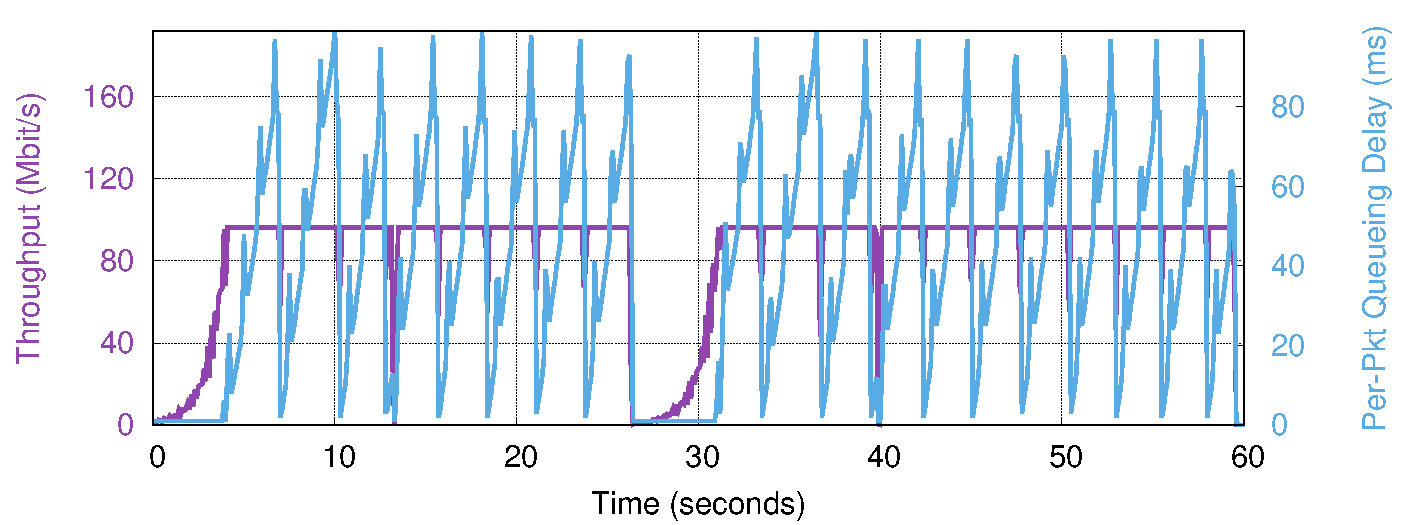
\includegraphics[width=\columnwidth]{img/bbr}
    \caption{
    Our CCP implementation of BBR used for a bulk transfer over a 96 Mbit/s link with a 100 ms RTT. The bandwidth probe phase can be seen in the oscillation of the queueing delay, and the RTT probe phase can be seen in the periodic dips in throughput.
    }\label{fig:ccp:bbr}
\end{figure}

We discuss how CCP allows a designer to focus on the essential features of their algorithm by outlining the implementation of BBR~\cite{bbr}. BBR is a rate-based scheme that models the network as a single bottleneck link. The sender probes for bandwidth in pulses of $1.25\times$ and $0.75\times$ of the current rate, setting its estimate of the bottleneck rate to a 10-second windowed maximum of the observed rate. If no new minimum RTT is reported for 10 seconds, BBR probes the minimum RTT by briefly draining the queue. BBR caps the congestion window to a fixed multiple (\texttt{cwnd\_gain}; recommended value is 2) of the ``pipe size'' (the product of the observed minimum RTT and estimated link rate). 

BBR is expressed succinctly with this control pattern:
\begin{minted}{rust}
  SetRateAbs(1.25 * bottleneck_estimate) =>
  SetCwndAbs(bottleneck_estimate * min_rtt
    * cwnd_gain) =>
  WaitRtts(1.0) =>
  SetRateAbs(0.75 * bottleneck_estimate) => 
  WaitRtts(1.0) => 
  SetRateAbs(bottleneck_estimate)
\end{minted}

Here, \texttt{bottleneck\_estimate}, \texttt{min\_rtt}, and \texttt{cwnd\_gain} are variables maintained in the CCP algorithm code, while the \texttt{Set...} and \texttt{WaitRTT} functions are interfaces provided by the datapath. 

To estimate the bottleneck rate, BBR uses a windowed maximum observed rate. For this purpose, the datapath must maintain estimates of the outgoing and incoming rates. The following fold function expresses how this signal as well as the minimum RTT are calculated: 
\begin{minted}{lisp}
(def 
    (Summary.bottleneck_estimate 0) 
    (Summary.minrtt +infinity))
(:= Summary.minrtt 
    (min Summary.minrtt A.rtt_sample_us))
(:= Summary.bottleneck_estimate 
    (max Flow.rate_outgoing Flow.rate_incoming))
\end{minted}

We implement the windowed min in the \texttt{OnReport()} handler in the CCP algorithm, not in the fold function. In Figure~\ref{fig:ccp:bbr}, we show the throughput and queueing delay achieved by our implementation.\footnote{We implemented only the bandwidth and RTT probing phases of BBR.} Both the characteristic BBR pulse, achieved from the control pattern, and the 10-second periodic probe-RTT mode, are evident.

%\subsection{Modular Design}
%\label{s:ccp:modular}
%\an{I'm not convinced this subsection is a strong argument}\fc{I feel the same. Maybe worth mentioning for those skeptical of difficulty, but perhaps a line or two as opposed to its own section?}
%
%\begin{outline}
%\begin{listing}
%{\footnotesize
%\begin{minted}{rust}
%fn linear_update(alpha, beta, cwnd) -> u32 {
%    return alpha * cwnd + beta;
%}
%fn additive_increase(cwnd) -> u32 {
%    return linear_update(1, 1/rtt, cwnd);
%}
%fn multiplicative_decrease(cwnd) -> u32 {
%    return linear_update(0.5, 0, cwnd);
%}
%\end{minted}
%}
%\caption{We implement a convenience layer atop the CCP API so users can build algorithms in a modular way.} \label{lst:modular}
%\end{listing}
%
%
%\1 While users may choose to use the above low-level semantics, we also provide a convenience API with which users may easily build simple algorithms.
%\1 The family of binomial TCP algorithms~\cite{binomial} can easily be implemented with this layer.
%%\1 Algorithms should strive to write their logic in a modular way for easy code reuse.
%%\1 \an{what exactly do we want to say here? most datapath algorithm implementations can reuse code from other algorithms}
%\end{outline}

\subsection{Case Study: Slow Start}
\label{s:ccp:semantics}

Because algorithms no longer make decisions upon every ACK, CCP changes the way in which developers should think about congestion control, and correspondingly provides multiple implementation choices. As a result, new issues arise about where to place algorithm functionality. We discuss the involved trade-offs with an illustrative example: slow start.

%We illustrate this with two examples: multiplicative decrease upon a drop and slow start.
%\cut{
%\subsubsection{Multiplicative Decrease}
%\label{s:ccp:semantics:md}
%algorithms specify that the congestion window should be halved upon a drop.
%However, a naive CCP implementation of this specification, shown in Listing~\ref{lst:reno}, will tend to be too conservative because it reduces its window multiple times if multiple packets in a row are lost.
%Indeed, a more precise specification of a multiplicative decrease algorithm is that the congestion window should be halved once per window in which a loss occurred.
%
%\begin{listing}[t]
%{\footnotesize
%\begin{minted}{rust}
%fn create(...) {
%  datapath.install_fold(sock_id, "
%  (def (Summary.acked 0) (Summary.loss 0))
%  (:= Summary.acked (+ Summary.acked A.bytes_acked))
%  := Summary.loss (+ Summary.loss A.lost_pkts_sample))
%  := isUrgent (> Summary.loss 0))
%  ");
%}
%fn onReport(...) {
%  if report.get_field("Summary.loss") > 0 {
%      self.multiplicative_decrease();
%  }
%}
%\end{minted}
%}
%\caption{An overly conservative implementation of multiplicative decrease. If multiple packets in a single congestion window are lost, the window may be cut twice.} \label{lst:reno}
%\end{listing}
%
%CCP makes these semantics explicit. A CCP implementation of multiplicative decrease, shown in Listing~\ref{lst:reno-fix}, tracks the packets received out-of-order and only allows a second reduction in the congestion window once enough in-order packets have arrived to account for the window worth of out-of-order and lost packets.
%
%This CCP-ready multiplicative decrease algorithm is available as a CCP module. \an{assuming modules exist}
%
%\fc{Graph from mtcp showing 2 drops w/o cwnd deficit and 1 drop with, if space}
%
%\begin{listing}[t]
%{\footnotesize
%\begin{minted}{rust}
%fn create(...) {
%  datapath.install_fold(sock_id, "
%  (def (Summary.acked 0) (Summary.sacked 0) (Summary.loss 0))
%  (:= Summary.acked (+ Summary.acked A.bytes_acked))
%  (:= Summary.sacked (+ Summary.sacked A.packets_misordered))
%  (:= Summary.loss (+ Summary.loss A.lost_pkts_sample))
%  (:= isUrgent (> Summary.loss 0))
%  ");
%}
%fn onReport(...) {
%  let acked, sacked, loss = report.get_fields(...);
%  if loss == 0 && self.deficit == 0 {
%      return;
%  } else if self.deficit > 0 {
%      self.deficit += sacked + loss - acked;
%  } else {
%      self.multiplicative_decrease();
%  }
%}
%\end{minted}
%}
%\caption{By tracking \texttt{A.packets\_misordered}, this implementation avoids reducing the window unnecessarily.} \label{lst:reno-fix}
%\end{listing}
%}

Slow start is a widely used congestion control module in which a connection probes for bandwidth by multiplicately increasing its congestion window (\texttt{cwnd}) every RTT. Most implementations increment \texttt{cwnd} per ACK, either by the number of bytes acknowledged in the ACK, or by 1 MSS. With CCP, one way to implement slow start is to retain the logic entirely in the CCP algorithm code, and measure the size of the required window update with a fold function. We show an example in Listing~\ref{lst:ccp:ss}. This implementation strategy is semantically closest in behavior to native datapath implementations.

\begin{listing}[t]
{\footnotesize
\begin{minted}{rust}
fn create(...) {
  datapath.install_fold(sock_id, "
  (def (Summary.acked 0) (Summary.loss 0))
  (:= Summary.acked (+ Summary.acked A.bytes_acked))
  ");
  datapath.install_pattern(
    SetCwndAbs(init_cwnd) => WaitRtts(1.0) => Report());
}
fn onReport(...) {
  let acked = report.get_field("Summary.acked");
  self.cwnd += acked;
  datapath.install_pattern(
    SetCwndAbs(self.cwnd) => WaitRtts(1.0) => Report());
}
\end{minted}
}
\caption{A CCP implementation of slow start (ending slow start not shown).} \label{lst:ccp:ss}
\end{listing}

\begin{figure}
    \centering
    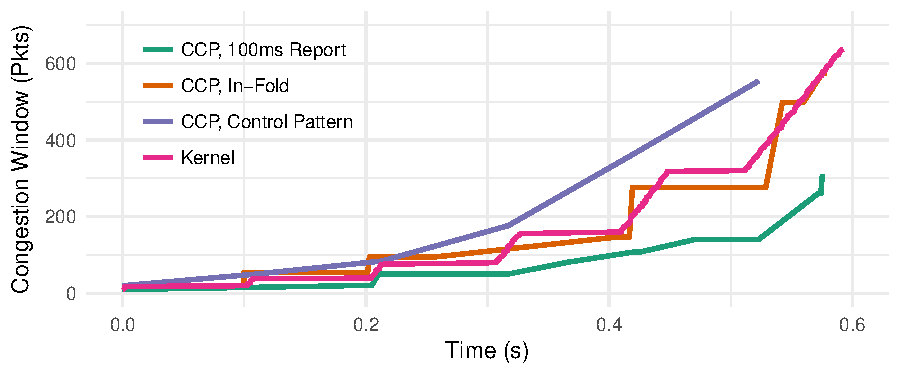
\includegraphics[width=\columnwidth]{img/ss-evo}
    \caption{Different implementations of slow start have different window update characteristics. The control pattern implementation is rate-based, so we show the congestion window corresponding to the achieved throughput over each RTT.}
    \label{fig:ccp:ss}
\end{figure}

For some workloads this approach may prove problematic, depending on the parameters of the algorithm. If the reporting period defined is large, then infrequent slow start updates can cause connections to lose throughput.
Figure~\ref{fig:ccp:ss} demonstrates, on a $48$ Mbps, $100$ ms RTT link, different implementations of slow start exhibit differing window updates relative to the Linux kernel baseline.
An implementation with a 1-RTT reporting period lags behind the kernel, but it is also possible to implement slow start within the fold function (Listing~\ref{lst:ccp:ssfold}), or in a control pattern: 

\begin{minted}{rust}
WaitRtts(1.0) => SetRateRel(2.0)
\end{minted}

As outlined in \S\ref{s:design}, the programming model of fold functions is deliberately limited.
First, we envision that in the future, CCP will support low-level hardware datapaths---the simpler the fold function execution environment is, the easier these hardware implementations will be. Second, algorithms able to make complex decisions on longer time-scales will naturally do so to preserve cycles for the application and datapath; as a result, complex logic inside the fold function may not be desirable.

Meanwhile, a control pattern is an easy way to program static behavior into the datapath, but is inflexible: CCP algorithms implementing slow start in a control pattern must be careful to exit slow start at the correct time; the control pattern will continue to scale the sending rate exponentially until it is replaced.

\smallskip

More broadly, developers may choose among various points in the algorithm design space. 
On one extreme, algorithms may be implemented almost entirely in CCP, using the fold function as a simple measurement query language.
On the other extreme, CCP algorithms may merely specify transitions between in-datapath fold functions implementing the primary control logic of the algorithm.
It is important to note, however, that some configurations, \eg making updates to the congestion window both in the fold function as well as via the send pattern makes the resulting algorithm difficult to reason about since the updates are not synchronized.
Ultimately, users will be able to choose the algorithm implementation best suited to their congestion control logic and application needs.

\begin{listing}[t]
{\footnotesize
\begin{minted}{rust}
fn create(...) {
  datapath.install_fold(sock_id, "
  (def (Summary.loss 0))
  (:= Cwnd (+ Cwnd A.bytes_acked))
  (:= isUrgent (> A.lost_packets 0))
  ");
}
fn onReport(...) {
  // exit slow start
}
\end{minted}
}
\caption{A within-fold implementation of slow start. Note that CCP algorithm code is not invoked at all until the connection experiences its first loss.} \label{lst:ccp:ssfold}
\end{listing}